\FloatBarrier
\section{Stage 3: Quantisation and error control}
Phase-0 measurements select the quantiser and code; a separate phase-1
study validates the frozen choices. All results use the supplied signal,
the R2 FIR and the receiver in Figure~\ref{fig:system-flow}.
\subsection{Resolution from measured SQNR and fidelity}
\label{sec:r31}
I select $ B=\QBits $, $ A=\QHalfRange $ and $\QLevels $ endpoint levels.
The endpoint scale--round--inverse mapping, extended by fixed scaling
and saturation, is 
\begin{align}
 z_c[n]&=\operatorname{clip}(z[n],-A,A),&
 v[n]&=z_c[n]/A,\qquad L=2^B,\\
 j[n]&=\operatorname{clip}\!\left(
 \operatorname{round}\!\left[\frac{v[n]+1-\epsilon}{2}(L-1)\right],
 0,L-1\right),\\
 z_q[n]&=A\left(\frac{2j[n]}{L-1}-1\right),
 \label{eq:r31mapping}\\
 q_j&=-A+\frac{2Aj}{L-1},&
 \Delta&=q_{j+1}-q_j=\frac{2A}{L-1}.
 \label{eq:r31spacing}
\end{align}
The implemented spacing is $2A/(2^B-1)$, whereas standard analysis uses
$\Delta_{\rm lec}=2A/2^B $.
I retain the fixed $\epsilon=10^{-9}$ and NumPy round-to-even.
The shifted granular bound is $|z_q-z_c|\le\Delta/2+A\epsilon $;
zero maps to $-\Delta/2 $, so exact zero bias is not assumed.
Appendix~\ref{app:quant} derives the codebook, headroom and error model.

The original signal already exceeds $[-1,1]$. Before drawing noise I fix
the same $ A=18 $ for filtered and unfiltered inputs over the declared
$-10 $ to 40 dB envelope. Six-standard-deviation headroom gives paired-record
overload bound $\QUnionBound $; it cannot guarantee no overload for an
unbounded Gaussian. Overloads are counted before clipping; none occurred
in the 80 branch records.
The measured implemented error-power ratio is
\begin{align}
 e_q[n]&=z_q[n]-z[n],\\
 P_z=\frac1N\sum_{n=0}^{N-1}z[n]^2,\qquad
 P_{e_q}&=\frac1N\sum_{n=0}^{N-1}e_q[n]^2,\\
 {\rm SQNR}_{\rm meas}&=10\log_{10}\frac{P_z}{P_{e_q}}.
 \label{eq:r31sqnr}
\end{align}
The uniform-error integral, $\Delta^2/12 $, and the ideal-model
$6.02B+1.76 $ full-range-sine special case are derived in
Appendix~\ref{app:quant}. They are models, not substitutes for the
measured error of this multitone/noisy input occupying part of a wide range.

\paragraph{Measured choice and cost.}
Five independent design records at each of eight SNRs
$\{-10,\allowbreak0,\allowbreak S_{\rm ID},\allowbreak10,\allowbreak20,\allowbreak30,\allowbreak35,\allowbreak40\}$, both filter settings and
$ B=4,\ldots,16 $ give 1040 measurements. The smallest acceptable width
must have no observed overload and satisfy the predeclared full-grid
component budget
\begin{equation}
 \rho_q(B)=\frac{\operatorname{mean}(q^2)}
                  {\operatorname{mean}(a^2)}
 \le0.01
 \quad\hbox{on every design record and both branches}.
 \label{eq:r31budget}
\end{equation}
Here $ a=\mathcal R(z)-u $ and $ q=\mathcal R(z_q)-\mathcal R(z)$ on all
96000 positions; the even-length Nyquist correction is
Eq.~\eqref{eq:r23-reconstruction-energy}. This 1 \% tolerance is a project
choice. Thirteen bits reaches \QPreviousPercent\%, while 14 reaches
 \QWorstPercent\%; the 40 dB no-filter case drives the limit.
Budgets 0.1/1/5 \% would select 16/14/13 bits, exposing the preference.

\begin{table}[htbp]
\centering\small
\caption{Fixed-range resolution/cost comparison. Worst component ratio includes both branches and all design records; SQNR is the anchor filtered result.}
 \label{tab:r31bits}
 \begin{tabular}{rrrrr}
\toprule
$B$ & Personal filtered SQNR & Worst component ratio & Payload & Pass \\
(bits) & (dB, mean of five) & (\%, 80 branch records) & (kbit/s) & 1\% budget \\
\midrule
8 & 26.551 & 2231.9352 & 128 & no \\
10 & 38.635 & 139.9707 & 160 & no \\
12 & 50.647 & 8.8692 & 192 & no \\
13 & 56.686 & 2.2218 & 208 & no \\
14 & 62.715 & 0.5586 & 224 & yes \\
15 & 68.732 & 0.1391 & 240 & yes \\
16 & 74.767 & 0.0347 & 256 & yes \\
\bottomrule
\end{tabular}



\end{table}


\begin{figure}[htbp]
\centering
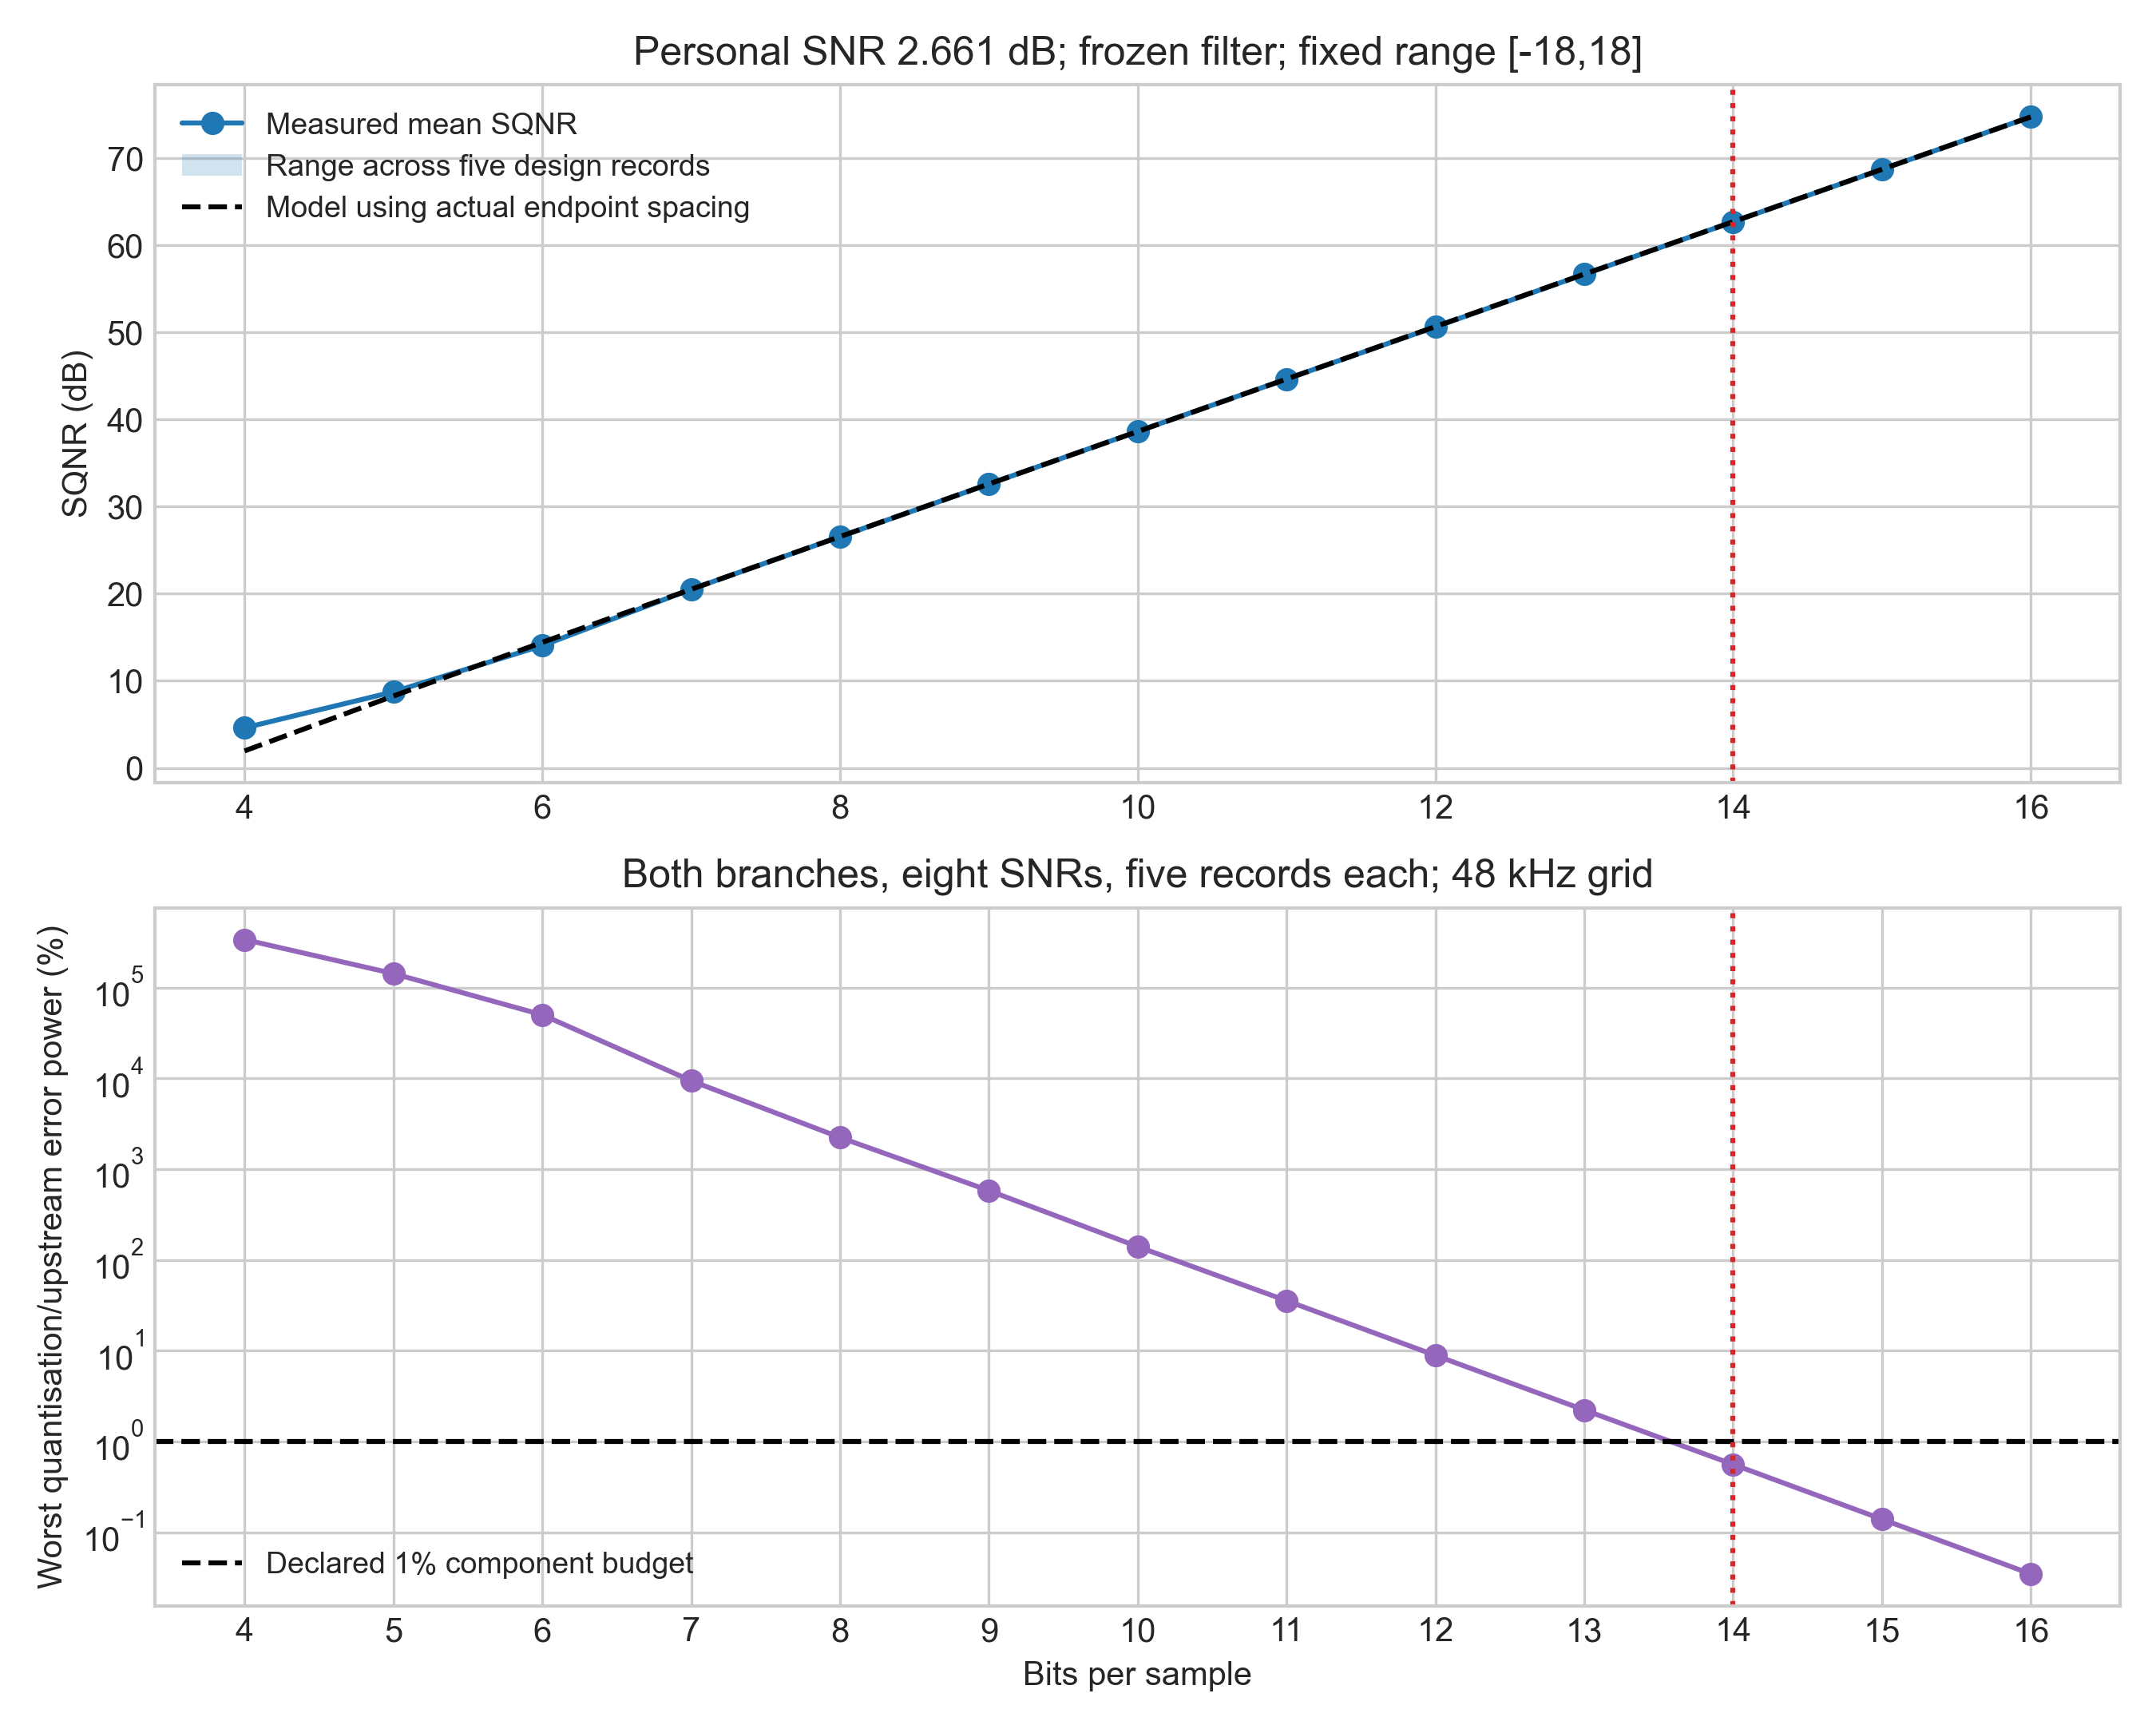
\includegraphics[width=.80\linewidth]{images/r31_sqnr_selection.png}
\caption{Measured SQNR and the declared component budget. Shading is the five-record design range, not a confidence interval; the low-bit model mismatch is retained.}
\label{fig:r31selection}
\end{figure}

At the anchor filtered point, measured SQNR is \QPersonalSqnr\,dB
(range [\QPersonalMin,\QPersonalMax]), model mean \QPersonalModel\,dB
and quantisation MSE $\QPersonalMse $. Complete-grid MSE changes from
$\QPersonalBefore $ to $\QPersonalAfter $. The 1 \% component budget permits
a 21 \% worst-case total-MSE change through cross terms
(Eq.~\eqref{eq:r31-total-bound}); the largest observed increase is
 \QMaxTotalPercent\%. A noisier input can have higher SQNR while being
less faithful to the reference, motivating the whole-chain metric in R4.

Fourteen bits uses 448000 information bits per record, 12.5 \% fewer than 16 bit.
Unsigned, sample-major, MSB-first packing is fixed; shared $ A,B $, length
and order are simulation metadata, not an assumed protected header.
All 131056 labels across the scanned widths round-trip, and independent
threshold quantisation/direct convolution/SciPy reconstruction reproduce
all 40 noise inputs and 1040 measurements. The quantiser freeze and
complete SQNR/error records remain under \path{stage3/r31/results/}.
